\chapter[Aboradagem de ER]{Aboradagem de ER}\label{cap3}

Nos dias atuais, a necessidade de automatização de processos se faz cada vez mais
presente. Processos são essenciais dentro de qualquer organização em qualquer área
de atuação, inclusive em uma das áreas mais recentes, que a produção de software.
A definição de processos de desenvolvimento de software vem com o objetivo de aumentar
a produtividade e diminuir os riscos de um projeto\cite{VIEIRA}.

Com o grande crescimento da demanda na produção de software
na atualidade os prazos estão cada vez mais curtos e cobrança relacionada a qualidade
estão cada vez maiores. A qualidade de um produto de software está diretamente ligada
a melhor forma de atender as necessidades do cliente, o que torna um produto totalmente dinâmico.
Uma vez que a natureza do produto é dinâmica existem grandes dificuldades no gerenciamento
do desenvolvimento, por exemplo: a essência volátil dos requisitos do cliente\cite{TAVARES}.

O produto de software também possui outra caracteristica única, é totalmente desenvolvido
por pessoas, o que gera outra gama de variáveis que podem causar risco e mudanças
imprevisíveis no meio de processo de produção \cite{SCHWABER}.

Com base nessas dificuldades, vários processo durante a história da Engenharia de
Software foram desenvolvidos, par amenizar esses problemas. Podemos citar destes
processos, os processos cascata, interativo, espiral, incremental

Considerando que para cada contexto de desenvolvimento um processo pode ser melhor
aplicado, para o a criação do processo de engenharia de requisitos adaptado aos
contextos da equipe, cliente e projeto, que serão aplicados nesse trabalho, foram
analisadas duas abordagens: Rational Unified Process(RUP) e o Scaled Agile Framework
Enterprise(SAFe). Será descrita uma breve introdução sobre ambos os processos e uma
juistificativa da escolha de atividades de cada um.

\section{Rational Unified Process}

O RUP foi criado pela Rational Software Corporation, é uma metodologia proprietaria,
que tem o objetivo de aumentar a produtividade focando na arquitetura do sistema
e na definição de seu processo, especificando regras e papéis\cite{IBM}.

Surgiu como uma abordagem inovadora pelo seu grande grau de customização, mas complexo,
recomendado para grandes equipes e grandes projetos \cite{KRUCHTEN}.

O RUP é composto por cinco componentes fundamentais:

\begin{enumerate}
  \item \textbf{Fluxos de trabalho}: É o passo a passo do que o envolvido deve seguir para
  desenvolver uma atividade.
  \item \textbf{Atividades}: Apresenta o trabalho que deve ser exercido por um membro da equipe
  apos está consciente do seu papel no decorrer do projeto.
  \item \textbf{Artefatos}: É o produto de trabalho de uma atividade, também pode servir de insumo para mesma.
  \item \textbf{Disciplinas}: É um conjunto de atividades que fazem parte de um mesmo grupo.
  \item \textbf{Papéis}: Apresenta a responsabilidade do envolvido em certa atividade
\end{enumerate}

A imagem abaixo ilustra um processo da engenharia de requistos na abordagem RUP.

\begin{figure}[H]
    \centering
  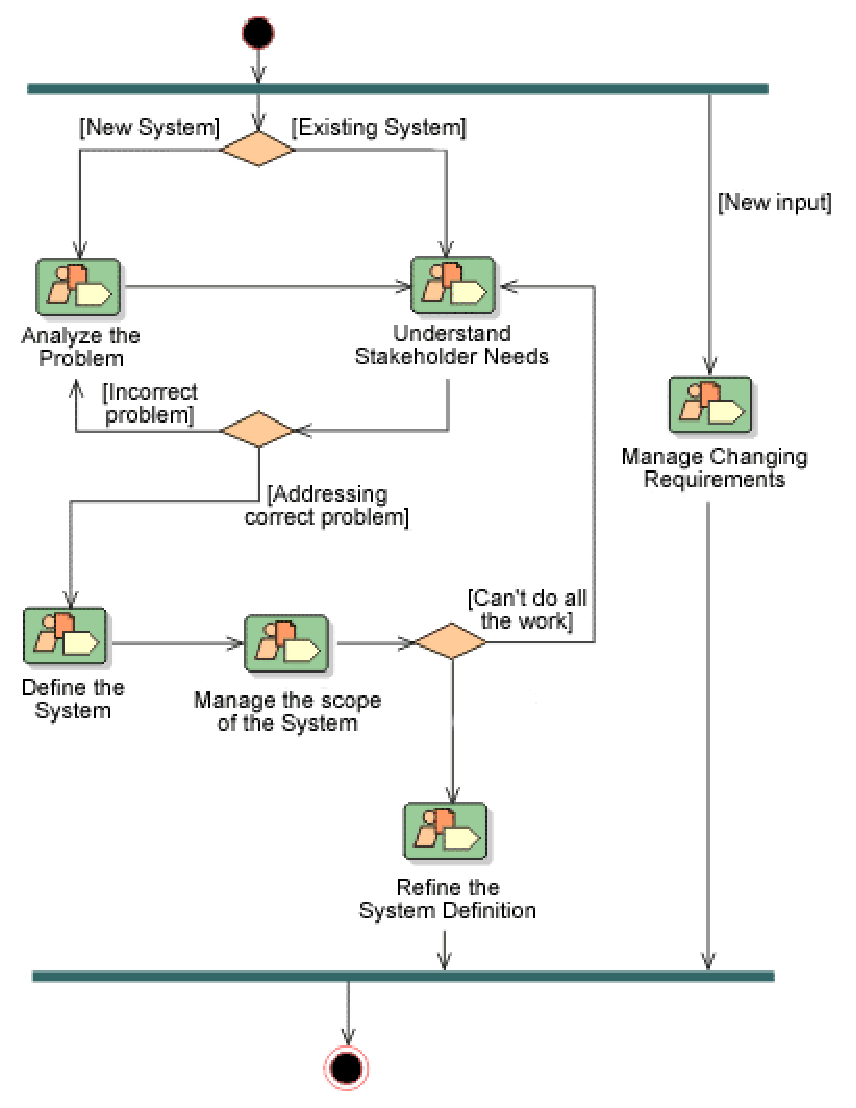
\includegraphics[keepaspectratio=true,scale=0.6]{figuras/WorkFlow_RUP_Requisitos.eps}
    \caption{Workflow do RUP}
    \label{fig:rup}
\end{figure}

\section{Scaled Agile Framework}

O SAFe é um processo enxuto, criado a partir das metodologias e filosofias ágeis,
que vieram como uma alternativa para criar entregas cada vez mais rápidas e alinhadas
as expectativas dos clientes, adaptando-se as constantes mudanças dos requisitos
e incertezas do cliente. Foi criado para se adaptar ao contexto empresarial.

O foco maior do SAFe é nas pessoas envolvidas no processo, e também no produto ao
inviés da documentação, tenta aproximar cada vez mais essas entidades. Colocam o
cliente com a posse do domínio do negócio e como membro da equipe o que influencia
na tomada de decisões durante o desenvolvimento do projeto.

Sendo assim, esse conjunto de práticas levam a maior adaptação a mudanças, possivelmente
amenizando os riscos na execução do projeto, pelo estreitamento entre a equipe do projeto
e o cliente \cite{BOEHM}.

O SAFe é composto por tres níveis organizacionais Portifólio(Estratégico),
Programa(Tático), Time(Operacional), como ilustrado na imagem \ref{fig:safe},e buscam seguir os seguintes princípios:

\begin{itemize}
  \item Adotar uma visão sistêmica
  \item Entendemos a economia da cadeia de valor
  \item Desenvolvemos sistemas iterativamente e incrementalmente
  \item Integramos e testamos frequentemente; adaptamos imediatamente
  \item Gerenciamos riscos e a eficácia através de ciclos de aprendizado rápido e síncrono
  \item Facilitamos o fluxo: limitamos o trabalho em execução, reduzimos o tamanho
  do lote e gerenciamos a duração da fila
  \item Sincronizamos entre os domínios o planejamento e a colaboração
  \item Baseamos marcos na avaliação objetiva dos sistemas de trabalho
  \item Desbloqueamos a motivação intrínseca dos trabalhadores do conhecimento
  \item Descentralizamos a tomada de decisão
\end{itemize}

\begin{figure}[H]
    \centering
  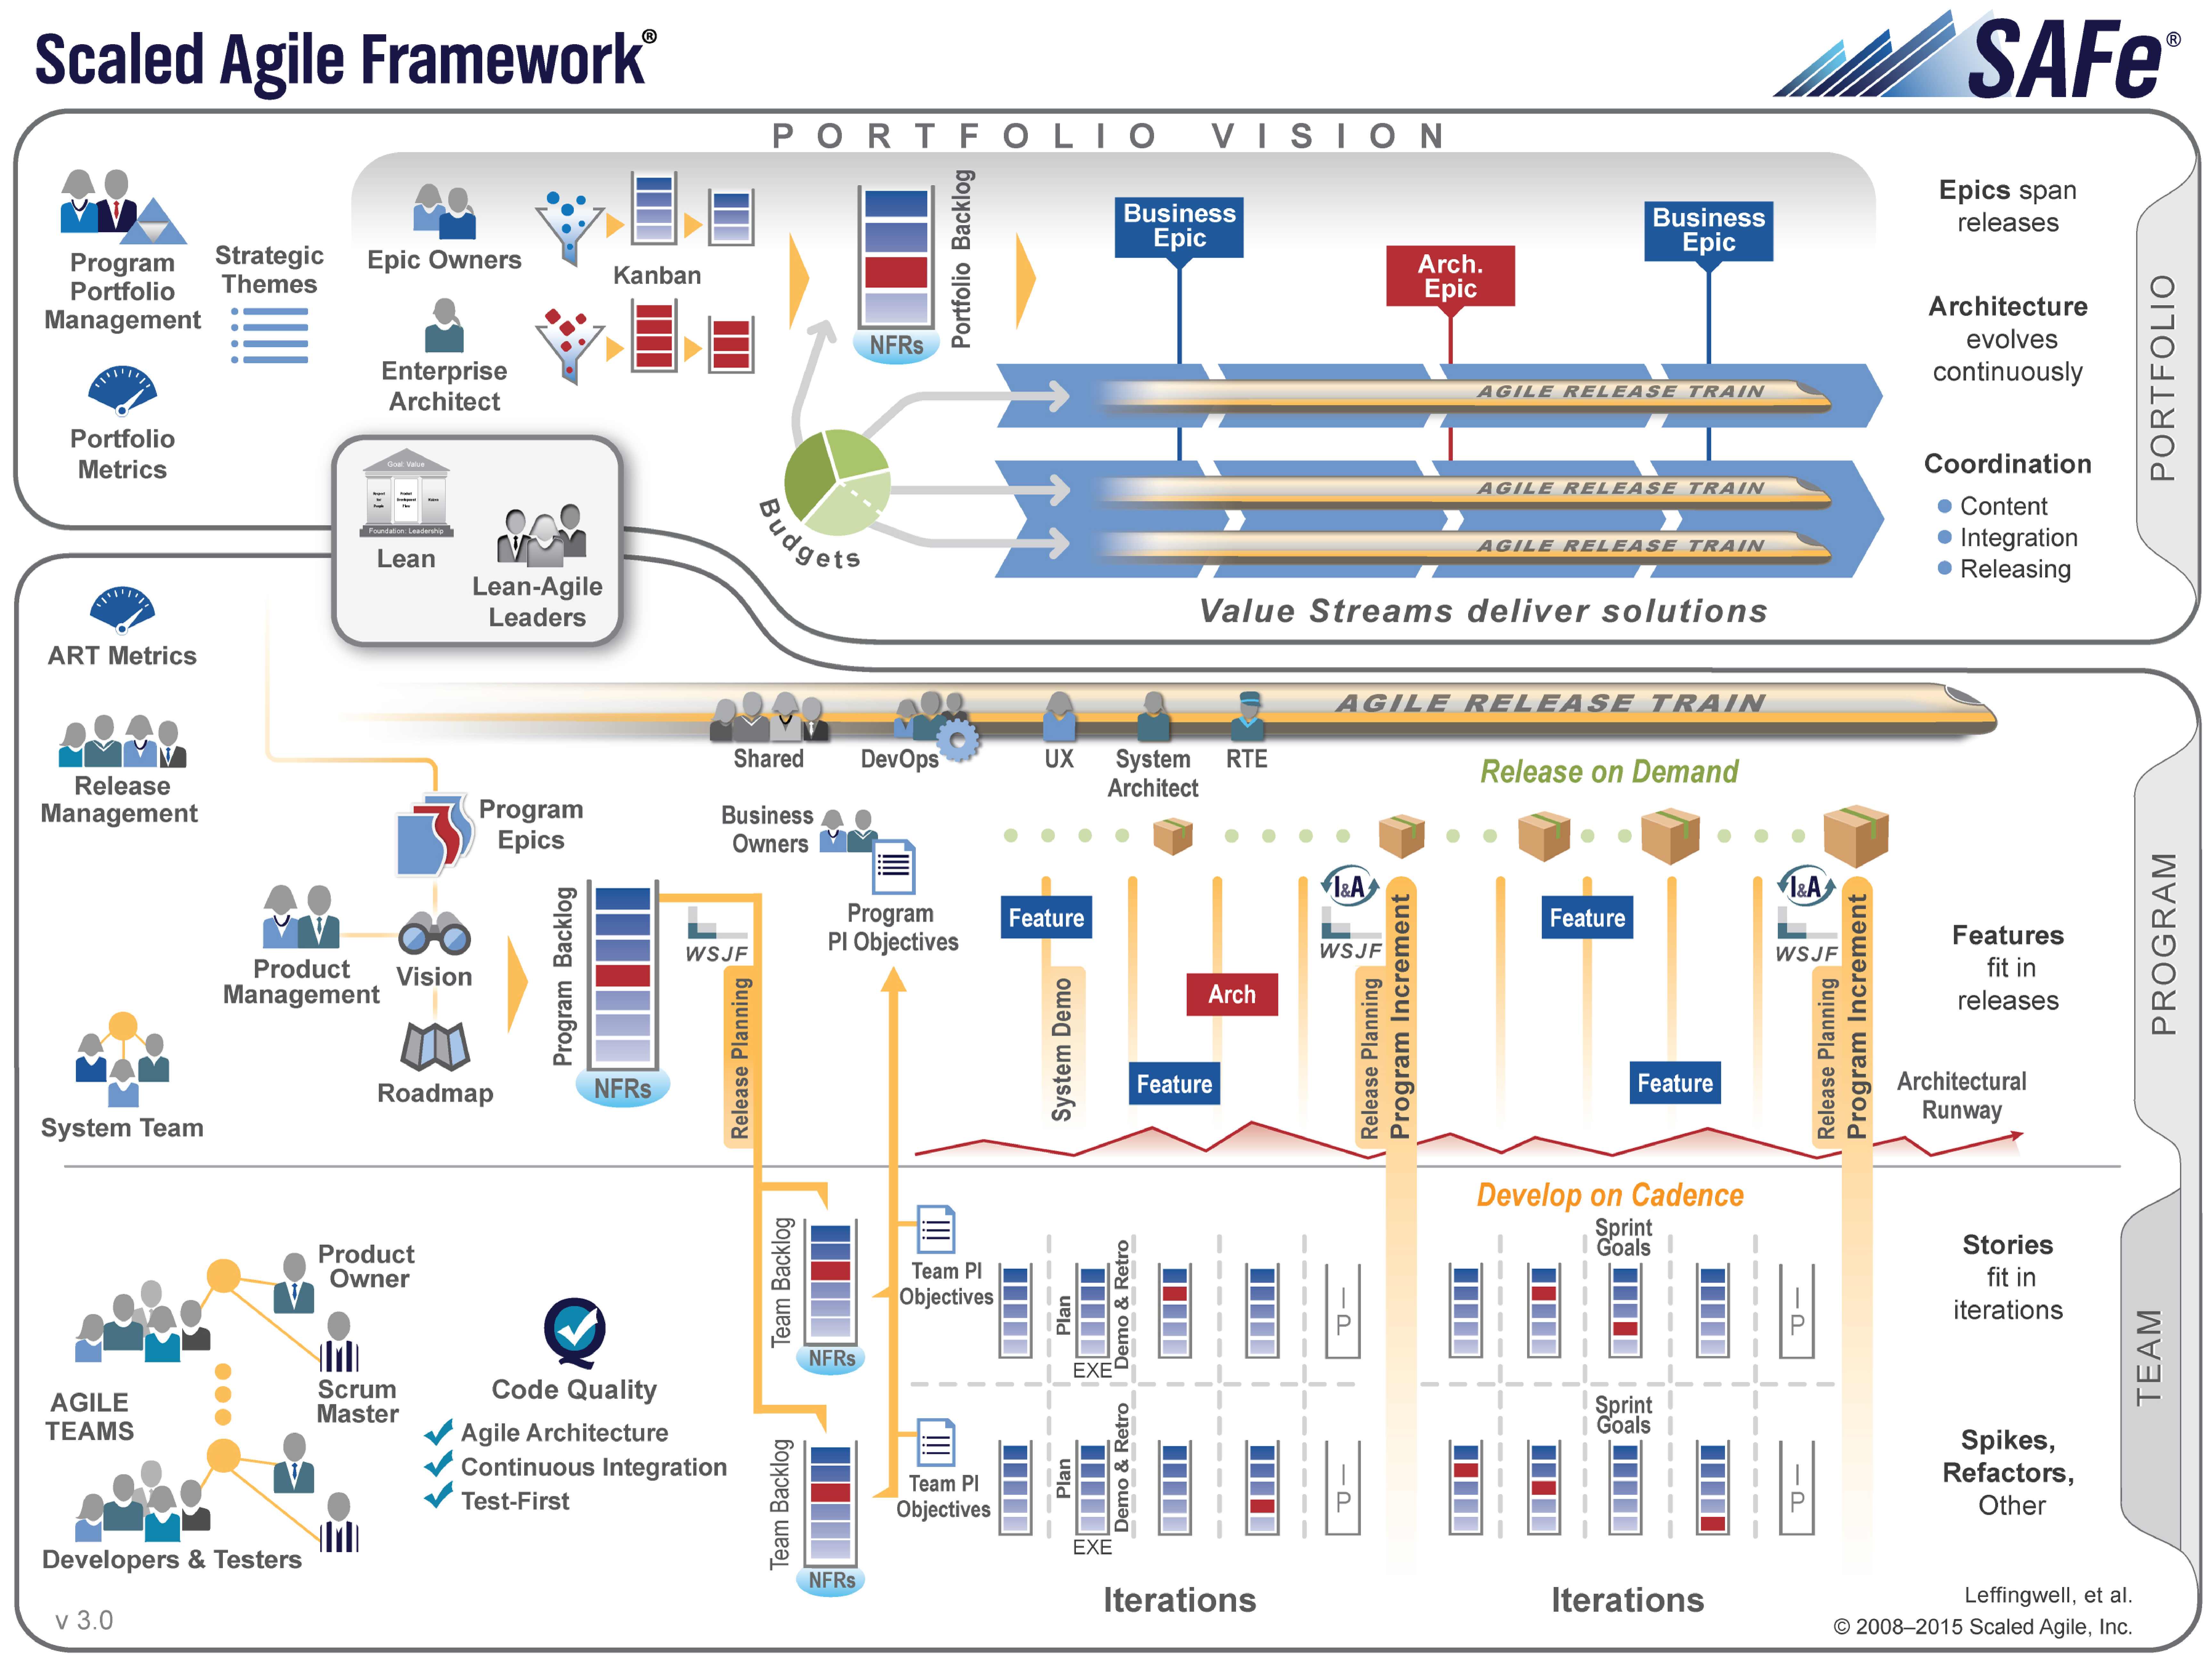
\includegraphics[keepaspectratio=true,scale=0.13]{figuras/SAFe_Big_Picture.eps}
    \caption{Visão geral do SAFe}
    \label{fig:safe}
\end{figure}

\section{Modelo de Maturidade}

Pode-se entender como conceito chave da maturidade de processos, a forma sistemática
a qual times considerados maduros realizam suas atividades, em comparação com o modo
de agir de times imaturos, que geralmente utilizam de abordagens criadas espontaneamente.

Em software, os modelo de maturidade são utilizados para:

\begin{enumerate}
  \item Avaliar o processo
  \item Melhoria de produtividade
  \item Melhoria contínua
\end{enumerate}

\subsection{Modelo CMMI}

O CMMI é um modelo que serve de base para o desenvolvimento e a avaliação da maturidade de uma organização.

O CMMI aborda a gerenciamento de requisitos, manipulação de riscos, medição de desempenho,
planejamento de trabalho e tomada de decisão.

No CMMI, um time pode escolher duas representações para a melhoria dos seus processos,
por estágio ou continua.

Em estágios, têm-se um caminho específico para a melhoria, como pode ser visto na figura seguinte:

\begin{figure}[H]
    \centering
  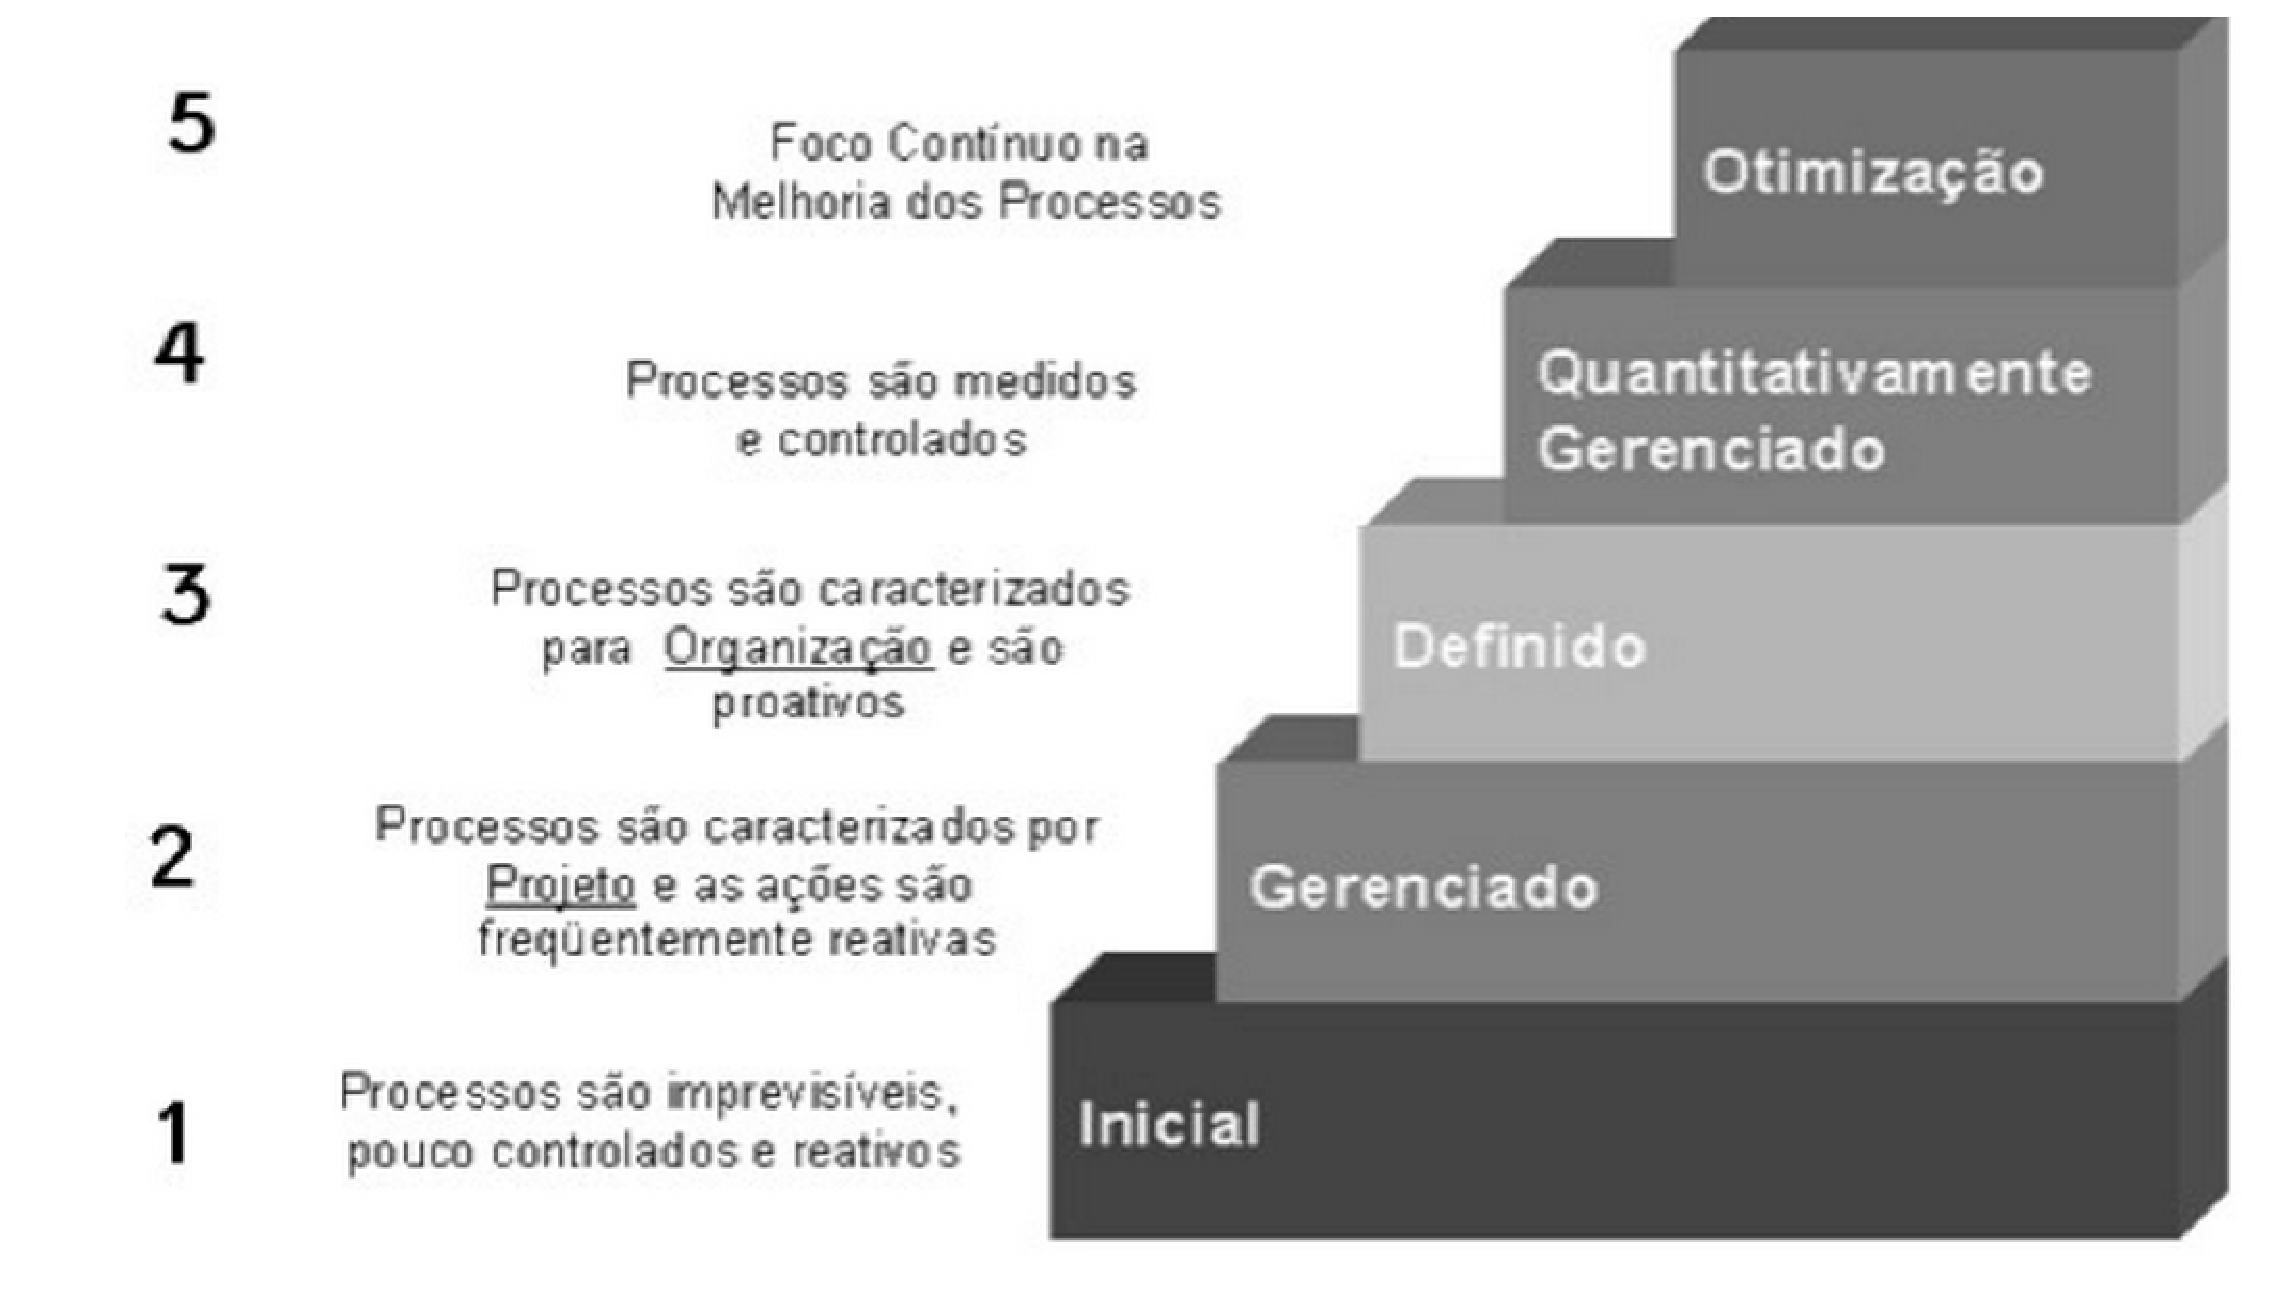
\includegraphics[keepaspectratio=true,scale=0.3]{figuras/cmmi.eps}
    \caption{Visão geral do CMMI}
    \label{fig:cmmi}
\end{figure}

\subsection{MPS.BR}

O modelo MPS-BR é dividido em níveis de maturidade, como ilustra a image x.

\begin{figure}[H]
    \centering
  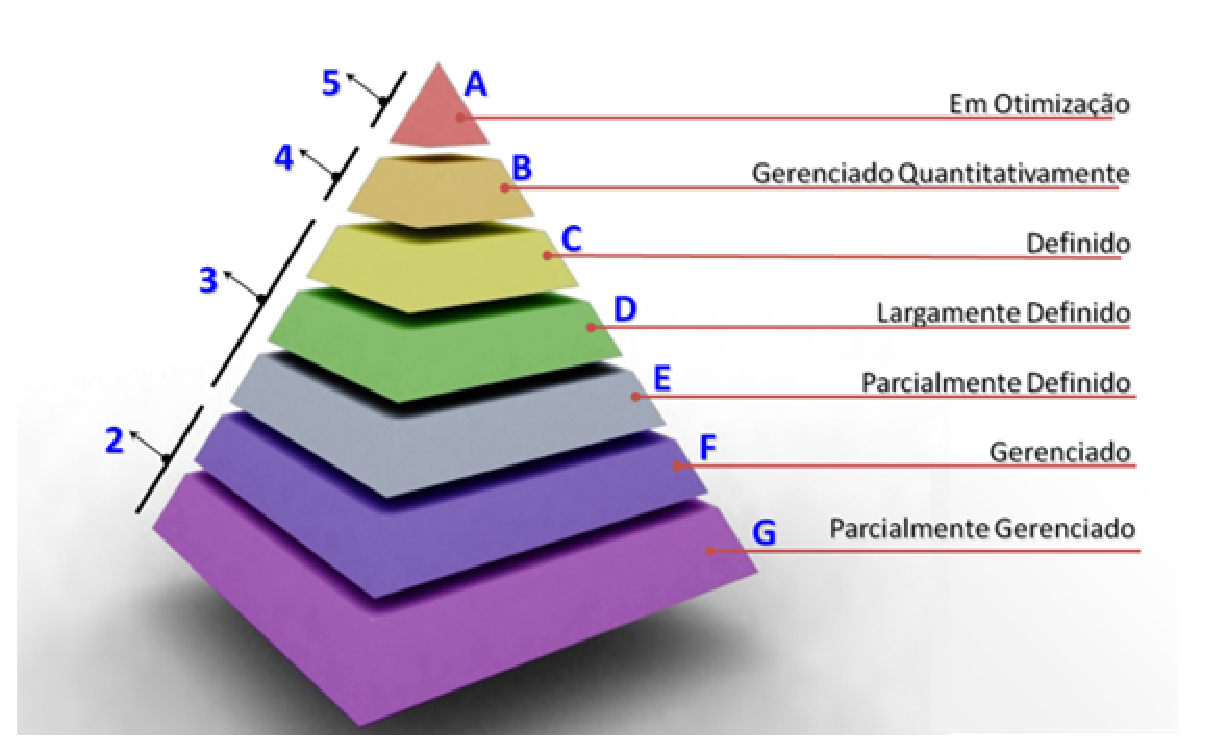
\includegraphics[keepaspectratio=true,scale=0.3]{figuras/mpsbr.eps}
    \caption{Visão geral do MPS.BR}
    \label{fig:mps}
\end{figure}

Cada nível de maturidade possui certas áreas de processos onde são analisados, sendo divididos
em três tipo.

\textbf{Processos Fundamentais}:
  \begin{itemize}
    \item Aquisição
    \item Gerência de requisitos
    \item Desenvolvimento de requisitos
    \item Solução técnica
    \item Integração do produto
    \item Instalação do produto
    \item Liberação do produto
  \end{itemize}


\textbf{Processos Organizacionais}:
\begin{itemize}
  \item Gerência de projeto
  \item Adaptação do processo para gerência de projeto
  \item Análise de decisão e resolução
  \item Gerência de riscos
  \item Avaliação e melhoria do processo organizacional
  \item Definição do processo organizacional
  \item Desempenho do processo organizacional
  \item Gerência quantitativa do projeto
  \item Análise e resolução de causas
  \item Inovação e implantação na organização
\end{itemize}

\textbf{Processos de Apoio}:
\begin{itemize}
  \item Garantia de qualidade
  \item Gerência de configuração
  \item Validação
  \item Medição
  \item Verificação
  \item Treinamento
\end{itemize}

Cada nível de maturação ainda apresenta uma quantidade de capacidades a serem analisadas

As engenharia de requisitos é abordada nos níveis G e D do MPS-BR, como Gerência de
Requisitos e Desenvolvimento de Requisitos respectivamente.

\begin{description}
  \item[Gerência de Requisitos] \hfill \\
  Busca gerenciar os requisitos do produto e do projeto, assim como identificar
  inconsistencias entre os requisitos, os planos de projeto e os produtos de trabalho do projeto.
  \item[Desenvolvimento de Requisitos] \hfill \\
  Busca definer os requisitos do cliente, do produto e dos components do produto.
\end{description}





\section{Mapeamento do Contexto vs Abordagens}

Considerando as duas influencias de abordagem foram levantadas as seguintes variáveis
relacionadas ao contextos do time, cliente, ambiente de trabalho, e projeto:

\begin{enumerate}
  \item \label{mapeamento:1} A equipe que trabalhará conta com apenas 5 membros, o que permite um
  auto-gerenciamento com mais facilidade, sendo de grande impacto definir um
  papel especifico apenas para algum membro cuidar do gerenciamento como é definido no RUP.
  \item A equipe atual já trabalhou com ambas as abordagens, e possui mais facilidade
  em implementar a abordagem ágil, devido a experiências anteriores.
  \item A equipe atual, é uma equipe que nunca trabalhou junta, o que pode ser um
  fator positivo para se escolher a abordagem tradicional, por ser mais específica
  e clara na descrição das atividades, e com documentação mais forte facilitando a comunicação.
  \item A equipe tem disponibilidade para encontros presenciais 4 vezes na semana
  e 7 vezes na semana por video conferência, o que facilita a implementação da abordagem ágil.
  \item A equipe não possui papeis específicos no projeto e nem uma hierarquia de
  responsabilidades, ou seja, há um compartilhamento de responsabilidades e espírito
  de colaboração, alinhado as práticas ágeis.
  \item O cliente possui grande disponibilidade por se encontrar no mesmo ambiente
  de trabalho da equipe, que é a Faculdade do Gama da Universidade de Brasília,
  o que facilita a aplicação da abordagem ágil que enfoca na participação ativa do cliente.
  \item O contexto do problema é criar software para otimizar algum gargalo no processo
  de uma organização, um requisito bem definido com possivelmente poucas mudanças.
  \item Em contrapartida o problema depende de uma terceira entidade que é o cliente
  do cliente, o que pode causar uma inconsistencia nas expectativas, assim o acompanhamento
  próximo do cliente é essencial para sucesso.
  \item O projeto possui um tempo limitado de 45 dias, um tempo consideravelmente curto,
  o que favorece a escolha da abordagem ágil que constituie-se em pequenas iterações,
  e também em menos burocracia para se adaptar as mudanças de requisitos.
\end{enumerate}

\section{Justificativa}

Para o desenvolvimento deste trabalho, foi definida uma abordagem híbrida.
Sendo sua base fundamental no SAFe e nas práticas ágeis levando em consideração
caracteristicas e atividades do RUP, uma vez que - como descrito na sessão 3.4
- os aspectos de equipe mapeados(\ref{mapeamento:1},2,4,5,6,7,8 e 9) com as abordagens bases
indicam que a utilização das práticas ágeis tornariam a execução do projeto mais
viável, porém o aspecto de equipe 3 apresenta um risco ao projeto caso não seja
devidamente utilizado no processo do projeto. Tornando assim evidente a necessidade
de uma abordagem híbrida.

Os modelos de maturidade abordados possuem diversas características em comum tanto nas fases
de implementação quanto nas fases organizacionais, as diferenças são apresentadas no que diz
respeito aos níveis de maturidade que são abordados em diferentes escalas quanto a medição e identificação.

No projeto em questão, optou-se por utilizar uma abordagem que seguisse o modelo de maturidade MPS-BR,
dentre as vantagens deste modelo em relação ao CMMI, pode-se citar que o MPS-BR é mais adequado a
realidade brasileira, além de ser focado em pequenas e médias empresas, encaixando-se
perfeitamente ao contexto presente.

O MPS-BR se torna muito mais acessível ao presente projeto em comparação ao CMMI,
que geralmente tem custo entre duzentos mil reais à um milhão de reais e requer um
certo tempo para se chegar aos níveis de maturidade mais altos.

Por outro lado, observa-se que a certificação MPS-BR não é suficiente para tornar
a equipe competitiva internacionalmente, fato que não prejudicará o time, visto sua
atuação somente no mercado brasileiro e no projeto em questão.

A partir dessa abordagem híbrida foi criado o processo descrito na sessão \ref{cap4}.
